\chapter{TERO-PUF: Concepts and general design}
\label{ch:concepts}

In this chapter, the concept behind \acrshort{teropuf}s will be discussed more in depth. In particular, how the randomness is exhibited using the \acrshort{tero} cells and how to generate the bit response from those them.

As we saw in chapter~\ref{ch:1-puf}, \acrshort{teropuf} is a delay-based \acrshort{puf}. It uses unstable oscillator circuits to exhibit the impact of the random defects in the \acrshort{ic}. In the following section, the two main parts of the \acrshort{teropuf} operation will be discussed: the \acrshort{tero} cell structure and the method to generate a response from them.

\section{TERO cells}
\label{sec:design_cells}

\begin{figure}[H]
    \centering
    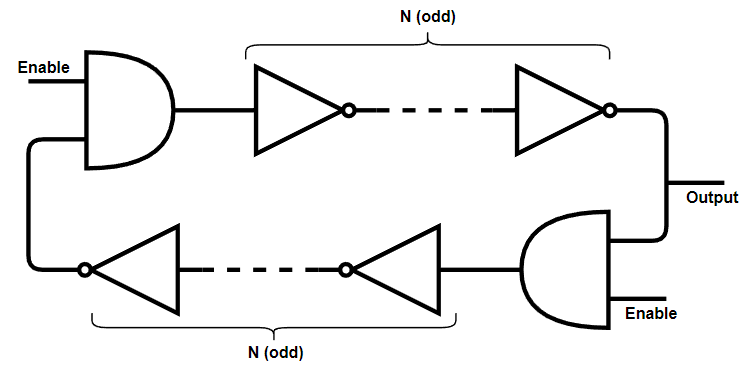
\includegraphics[width=0.55\linewidth]{images/tero_structure.png}
   \caption{\label{fig:cell_diagram}TERO cell logical representation}
\end{figure}

The structure of the \acrshort{tero} cell (represented in figure~\ref{fig:cell_diagram}) is related to the \acrshort{sr-latch} but where the \textit{set} and \textit{reset} inputs are used simultaneously (the \textit{enable} signal on the diagram). The two opposite AND gates serve as the entry point for the signals when the cell is enabled, and an equal and odd number of NOT gates on each branch create a delay inside the loop. The initial state (when \textit{enable} is low) is stable, as represented in figure~\ref{fig:ter_cell_states}(a).\\

Once \textit{enable} is set to high, this circuit becomes an oscillator with two signals propagating inside the loop, which toggles the output signal. Due to the imperfect nature of any real \acrshort{ic}, one signal will eventually catch up with the other, they will cancel each other, stopping the oscillation and reaching one of the two stable states, represented in figure~\ref{fig:ter_cell_states}(b). The final state depends on which signal catches the other. At this point, the cell will stay in this state until the \textit{enable} signal falls, which will reset the cell to the initial state through the AND gates. The number of NOT gates on each branch (noted N) is used as a parameter to choose the length of the propagation path inside the cell but needs to remain odd.\\

\begin{figure}[H]
   \begin{minipage}[b]{0.50\linewidth} 
        \centering
        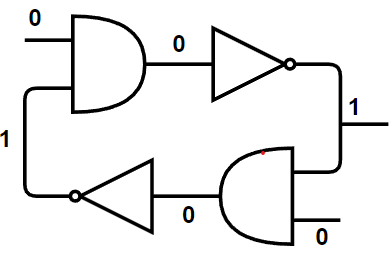
\includegraphics[width=0.6\linewidth]{images/tero_init_state.png}
        \subcaption{Initial state}
   \end{minipage}\hfill
   \begin{minipage}[b]{0.50\linewidth}   
        \centering
        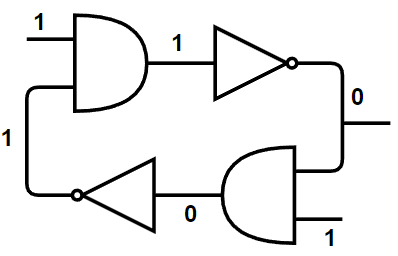
\includegraphics[width=0.6\linewidth]{images/tero_final_state.png}
        \subcaption{Final state}
   \end{minipage}
   \caption{\label{fig:ter_cell_states}\acrshort{tero} cell states (N=1)}
\end{figure}

The effect of the random defect of the \acrshort{ic} on this circuit can be observed in two ways: the final state reached after stabilisation and the number of oscillations reached before this stabilisation. These two properties can be used to generate bits from this structure.


\section{Response generation}
\label{sec:design_generation}


The PUF needs to generate a sequence of bits from the \acrshort{tero} cells, using either the final state or the final number of oscillations. To do so, the simplest method could consist of using the final state of the cell directly as the bit response since it has only two possible states. This is represented in the figure~\ref{fig:generative_meth_1}.\\

This has the advantage of being very simple to implement. However, the issue with this technique is that the cells need to be perfectly reliable or the bits would not be stable. It has been shown in~\cite{bossuet_puf_2014, marchand_implementation_2017} that some cells take much more time to stabilise, to the point where they can be considered as "unstable" and will produce an unreliable bit. An additional drawback is that the number of bits that can be generated is equal to the number of \acrshort{tero} cells. Therefore, the resource usage for this method scales linearly with the size of the response. \\



\begin{figure}[H]
   \begin{minipage}[b]{0.47\linewidth} 
        \centering
        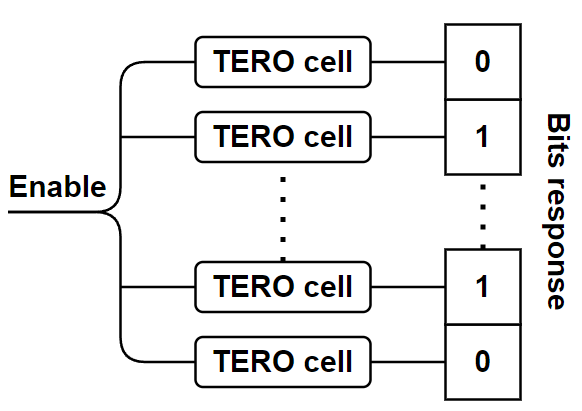
\includegraphics[width=\linewidth]{images/generative_meth_1.png}
        \subcaption{Direct\label{fig:generative_meth_1}}
   \end{minipage}\hfill
   \begin{minipage}[b]{0.53\linewidth}   
        \centering
        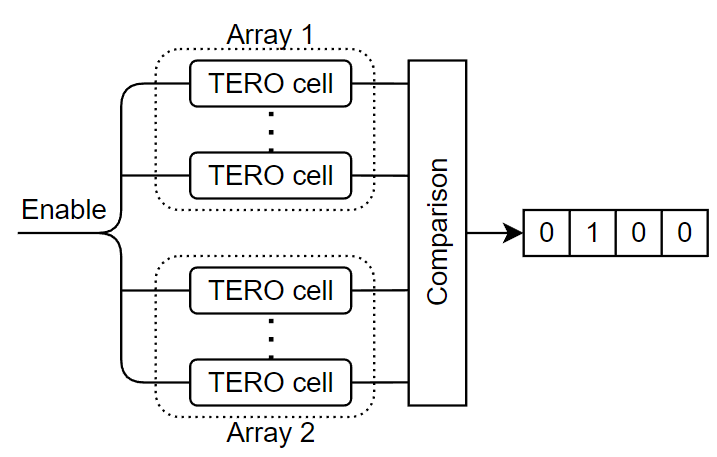
\includegraphics[width=\linewidth]{images/generative_meth_2.png}
        \subcaption{Comparison\label{fig:generative_meth_2}}
   \end{minipage}
   \caption{Bit generation method}
\end{figure}


Another approach (represented in figure~\ref{fig:generative_meth_2}) is to compare the number of oscillations of two cells after stabilisation. A '1' is generated if the first cell has a higher number of oscillations, and a '0' is generated otherwise. This is the method used by~\cite{de_weerdt_implementation_2021}.\\

This method is less sensitive to the cell's exact number of oscillations in terms of the reliability of the response as long as the number of oscillations of the different cells is clearly spread. By splitting K cells into two arrays for the comparison, the number of bits that can be generated is equal to $\left ( \frac{K}{2}\right )^2$. This scales quadratically with the size of the response, which is better than the first method. One can notice that equality between the two cells will always generate a '0' in this method. This could degrade the uniformity of the response if too many equalities occur and this is something that will need to be tested once the \acrshort{puf} is implemented.\\


A third design, the gray coding response generation, used in~\cite{marchand_implementation_2017}, is to subtract the number of oscillations of two cells, apply a Gray coding on this value then select specific bits from this code to create a part of the response. 
This has the disadvantage that the bits need to be analysed to determine which ones are the more stable in order to select them to generate a chip ID that is reliable. This also adds additional elements to the design compared to the second method.

\begin{figure}[H]
    \centering
    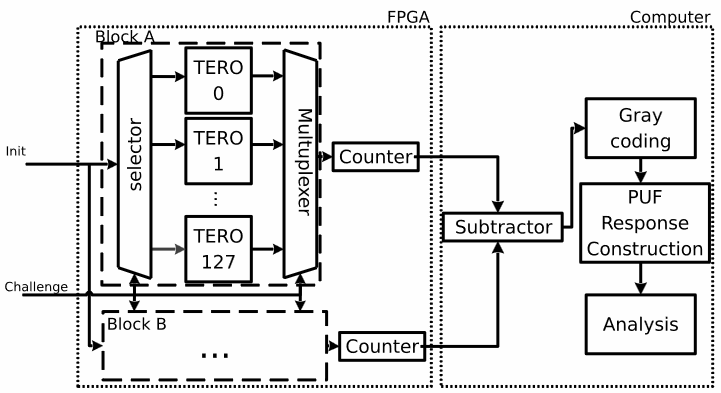
\includegraphics[width=0.75\linewidth]{images/tero_gray_coding.png}
    \caption{Gray coding response generation (figure from~\cite{marchand_implementation_2017})}
    \label{fig:generative_meth_3}
\end{figure}

The second method is chosen because it has a small footprint while producing a response with good reliability. Furthermore, it also ensures higher compatibility with the implementation of~\cite{de_weerdt_implementation_2021}.\\

To maximise the size of the response, each cell should be compared to every cell of the opposite array. Instead of storing all the possible combinations in memory,~\cite{de_weerdt_implementation_2021} has proposed to use a \acrfull{lsfr} circuit to compute them as needed. Indeed, a such circuit will cycle through the entire possible $2^{N} -1$ values exactly once before returning to the initial state (where N is the size of the register). The first half bits of the \acrshort{lsfr} can be used as a selection for the first array, and the remaining bits for the second array.

This way, all the possible combinations are covered except the 0-0 one because the state with only '0' is a forbidden state (the \acrshort{lsfr} would stay in this state forever), reducing the size of the response bit one. For a large enough number of cells, this impact will become negligible. Moreover, this implementation takes very little hardware resources and scale better than storing all the combination in memory. For those reasons, this \acrshort{lsfr} will also be used in this implementation. The new size of the \acrshort{puf} response is therefore equal to $\left ( \frac{K}{2}\right )^2 -1$.

\begin{figure}[H]
    \centering
    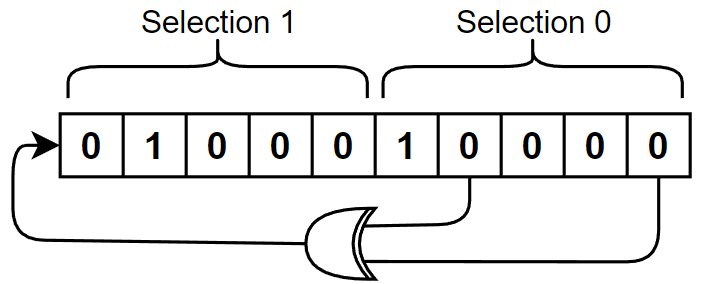
\includegraphics[width=0.5\linewidth]{images/LSFR.png}
    \caption{10-bits \acrshort{lsfr}}
    \label{fig:LSFR}
\end{figure}

\section{TERO-PUF operation}
\label{sec:design_operation}

We can now fully describe the operation of our \acrshort{teropuf}: the \acrshort{tero} cells are composed of 2 AND gates and $2\times N$ NOT gates (N is odd). K cells are split into two arrays (K need to be even). Each possible pair (except the '0-0' one) is selected in turn using an \acrshort{lsfr}. For each pair, the two selected cells are enabled at the same time along with a reference counter connected to the clock, and the number of oscillations is recorded. Once the reference counter reaches the number of clock cycles corresponding to the desired acquisition time, the number of oscillations is compared and one bit of the response is generated. Then the cells and the reference counter are disabled, which reset their state, and the \acrshort{lsfr} is shifted to generate the next combination to be selected. $\left ( \frac{K}{2}\right )^2 -1$ bits are generated in this way. The usage of the reference counter imposes that the acquisition time can only be a multiple of the clock period ($\frac{1}{f}$)\\


\begin{figure}[H]
    \centering
    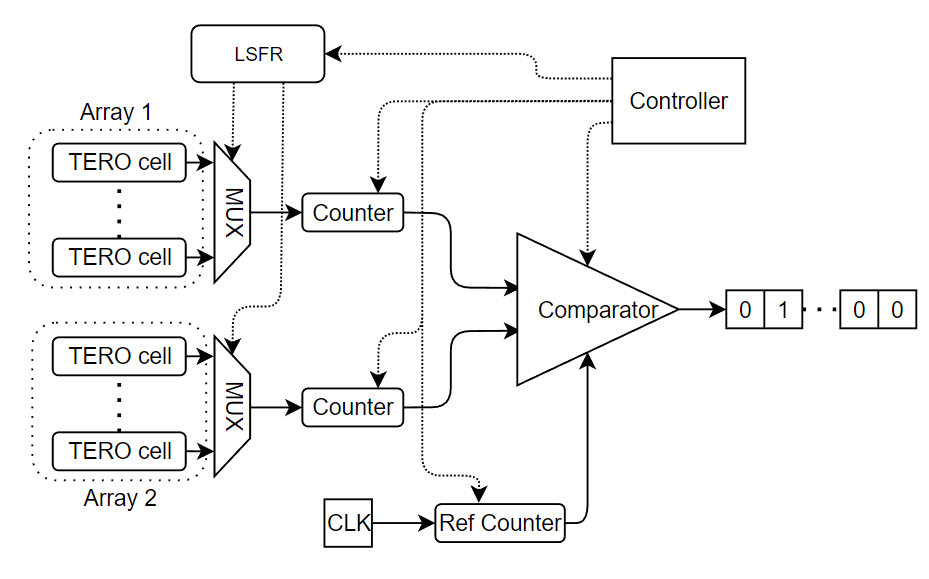
\includegraphics[width=1\linewidth]{images/puf_block.png}
    \caption{\acrshort{teropuf} block diagram}
    \label{fig:generative_sum}
\end{figure}

